\pdfinfoomitdate=1
\pdftrailerid{}
\pdfsuppressptexinfo=-1
\documentclass[10pt,a4paper]{article}
\usepackage{cmap}
\usepackage[margin=1.8cm,headheight=14pt,headsep=10pt]{geometry}
\usepackage[leqno]{amsmath}
\usepackage{amssymb,booktabs,longtable,array,ragged2e,multicol,multirow,xcolor,fancyhdr,tikz}
\definecolor{linkblue}{rgb}{0.08,0.33,0.58}
\usepackage[colorlinks=true,linkcolor=linkblue,urlcolor=linkblue,citecolor=linkblue,
  filecolor=linkblue,linktoc=all,pdfborder={0 0 0},bookmarksnumbered=true]{hyperref}
\setlength{\parindent}{0pt}\setlength{\parskip}{4pt}
\setcounter{secnumdepth}{2}\setcounter{tocdepth}{2}
\definecolor{partshade}{gray}{0.9}
\definecolor{parttitle}{HTML}{7A1466}
\definecolor{parttitlelight}{HTML}{D66EBC}
\makeatletter
\renewcommand\section{\@startsection{section}{1}{\z@}{-3ex plus -1ex minus -.2ex}%
  {1.2ex plus .2ex}{\normalfont\large\sffamily\bfseries\color{parttitle}}}
\renewcommand\subsection{\@startsection{subsection}{2}{\z@}{-2.5ex plus -1ex minus -.2ex}%
  {.8ex plus .2ex}{\normalfont\sffamily\bfseries\color{parttitle}}}
\renewcommand\subsubsection{\@startsection{subsubsection}{3}{\z@}{-2ex plus -1ex minus -.2ex}%
  {.6ex plus .2ex}{\normalfont\small\sffamily\bfseries\color{parttitle}}}
\renewcommand\paragraph{\@startsection{paragraph}{4}{\z@}{1.5ex plus .5ex minus .2ex}{-1em}%
  {\normalfont\small\sffamily\bfseries\color{parttitle}}}
\renewcommand\tagform@[1]{\maketag@@@{\textsf{\bfseries\footnotesize (#1)}}}
\renewcommand*\l@part[2]{\par\addvspace{1.6ex}\noindent{\sffamily\bfseries #1}\hfill
  {\sffamily\bfseries #2}\par\nobreak}
\newcommand\tocnumber{1.8em}
\newcommand\tocline[4]{\par{\rightskip \tocnumber plus 1fil\relax\parfillskip -\rightskip
  \noindent\hangindent\dimexpr#1+#2\relax\hspace*{#1}%
  \@tempdima #2{\sffamily\small #3}\nobreak\leaders\hbox{$\m@th\mkern 4.5mu\hbox{.}%
  \mkern 4.5mu$}\hfill\nobreak\hbox to \tocnumber{\hfil\sffamily\small #4}\par}}
\renewcommand*\l@section[2]{\tocline{0em}{2.2em}{#1}{#2}}
\renewcommand*\l@subsection[2]{\tocline{2.2em}{2.6em}{#1}{#2}}
\newcommand\contentspage{{\setlength{\columnsep}{24pt}\begin{multicols}{2}\@starttoc{toc}%
  \end{multicols}}}
\newcounter{docpart}\@addtoreset{section}{docpart}
\renewcommand\thesection{\ifnum\value{docpart}>0 \arabic{docpart}.\fi\arabic{section}}
\renewcommand\theHsection{\arabic{docpart}.\arabic{section}}
\newcommand\partnumber[1]{#1\enspace}
\pdfstringdefDisableCommands{\def\partnumber#1{#1 }}
\newcommand{\partbox}[1]{\par\addvspace{12pt}\refstepcounter{docpart}\phantomsection
  \addcontentsline{toc}{part}{\protect\partnumber{\thedocpart}#1}%
  \noindent\colorbox{partshade}{\makebox[%
  \dimexpr\textwidth-2\fboxsep\relax]{\rule[-6pt]{0pt}{20pt}\Large\sffamily\bfseries%
  \textcolor{parttitle}{\thedocpart\quad #1}}}\par\nobreak\@nobreaktrue\addvspace{2pt}}
\newmarks\LTstartmarks\newcount\LTstartcount
\let\LT@startplain\LT@start
\def\LT@start{\global\advance\LTstartcount\@ne\LT@startplain
  \marks\LTstartmarks{\the\LTstartcount}}
\newmarks\LTgroupmarks
\newcount\LTspacebreak\LTspacebreak=-1
\newcount\LTrulebreak\LTrulebreak=-2
\def\grouprule#1#2{\noalign{\marks\LTgroupmarks{\the\belowrulesep}\nobreak\vskip#1%
  \vskip\aboverulesep}\multispan\LT@cols\unskip{\leaders\hrule\@height#2\hfill\kern\z@}\cr
  \noalign{\penalty\LTrulebreak\vskip\belowrulesep\global\@lastruleclass\z@}}
\def\groupspace#1{\noalign{\marks\LTgroupmarks{\the\dimexpr#1\relax}\penalty\LTspacebreak
  \vskip#1\global\@lastruleclass\z@}}
\def\LT@unskips{\unskip\unpenalty\unskip\unpenalty\unskip\unpenalty\unskip\unpenalty}
\def\LT@groupcut{\ifnum\outputpenalty=\LTrulebreak
  \setbox\@cclv\vbox{\unvbox\@cclv\setbox\z@\lastbox\LT@unskips}\fi}
\def\LT@groupjoin{\ifnum\outputpenalty=\LTspacebreak\vskip-\botmarks\LTgroupmarks\relax\fi
  \ifnum\outputpenalty=\LTrulebreak\vskip-\botmarks\LTgroupmarks\relax\fi}
\let\LT@outputplain\LT@output
\def\LT@output{\ifnum\outputpenalty<-\@Mi\LT@outputplain\else
  \edef\LT@marka{\botmarks\LTstartmarks}\edef\LT@markb{\the\LTstartcount}%
  \ifx\LT@marka\LT@markb\LT@groupcut\LT@outputplain\LT@groupjoin
  \else\setbox\LT@head\box\voidb@x\LT@outputplain\fi\fi}
\makeatother
\newcommand{\needspace}[1]{\par\penalty-100\begingroup\dimen0=#1\relax\dimen2=\pagegoal
  \advance\dimen2-\pagetotal\ifdim\dimen0>\dimen2\relax\ifdim\dimen2>0pt\vfil\break\fi\fi
  \endgroup}
\numberwithin{equation}{section}
\pagestyle{fancy}\fancyhf{}
\renewcommand{\headrulewidth}{0pt}
\renewcommand{\sectionmark}[1]{\markright{\thesection\enspace #1}}
\renewcommand{\subsectionmark}[1]{}
\fancyhead[R]{\small\textsc{\rightmark}\quad\thepage}
\fancypagestyle{plain}{\fancyhf{}\fancyfoot[C]{\small\thepage}}
\definecolor{atlasI}{HTML}{991A1A}\definecolor{atlasIl}{HTML}{EC6B60}
\definecolor{atlasII}{HTML}{295A2C}\definecolor{atlasIIl}{HTML}{6C9F6D}
\definecolor{atlasIII}{HTML}{7A1466}\definecolor{atlasIIIl}{HTML}{D66EBC}
\definecolor{atlasIV}{HTML}{9B690B}\definecolor{atlasIVl}{HTML}{F2A618}
\makeatletter
\newcommand\atlas@full{%
\fill[atlasIII] (0.0394,0.0163) -- (0.3978,0.0163) arc[start angle=0.668, end angle=13.836, radius=1.3979] -- cycle;
\fill[atlasI] (-0.0163,0.0394) -- (-0.0163,0.3978) arc[start angle=90.668, end angle=103.836, radius=1.3979] -- cycle;
\fill[atlasIV] (-0.0394,-0.0163) -- (-0.3978,-0.0163) arc[start angle=-179.332, end angle=-166.164, radius=1.3979] -- cycle;
\fill[atlasII] (0.0163,-0.0394) -- (0.0163,-0.3978) arc[start angle=-89.332, end angle=-76.164, radius=1.3979] -- cycle;
\fill[atlasIIIl] (0.0163,0.0394) -- (0.3343,0.3573) arc[start angle=76.164, end angle=89.332, radius=1.3979] -- cycle;
\fill[atlasIl] (-0.0394,0.0163) -- (-0.3573,0.3343) arc[start angle=166.164, end angle=179.332, radius=1.3979] -- cycle;
\fill[atlasIVl] (-0.0163,-0.0394) -- (-0.3343,-0.3573) arc[start angle=-103.836, end angle=-90.668, radius=1.3979] -- cycle;
\fill[atlasIIl] (0.0394,-0.0163) -- (0.3573,-0.3343) arc[start angle=-13.836, end angle=-0.668, radius=1.3979] -- cycle;
\fill[atlasIIIl] (0.4304,0.0163) -- (0.9598,0.0163) arc[start angle=46.637, end angle=73.849, radius=1.3979] arc[start angle=13.862, end angle=0.653, radius=1.4305] -- cycle;
\fill[atlasIl] (-0.0163,0.4304) -- (-0.0163,0.9598) arc[start angle=136.637, end angle=163.849, radius=1.3979] arc[start angle=103.862, end angle=90.653, radius=1.4305] -- cycle;
\fill[atlasIVl] (-0.4304,-0.0163) -- (-0.9598,-0.0163) arc[start angle=-133.363, end angle=-106.151, radius=1.3979] arc[start angle=-166.138, end angle=-179.347, radius=1.4305] -- cycle;
\fill[atlasIIl] (0.0163,-0.4304) -- (0.0163,-0.9598) arc[start angle=-43.363, end angle=-16.151, radius=1.3979] arc[start angle=-76.138, end angle=-89.347, radius=1.4305] -- cycle;
\fill[atlasIII] (0.0163,0.4304) arc[start angle=89.347, end angle=76.138, radius=1.4305] arc[start angle=16.151, end angle=43.363, radius=1.3979] -- cycle;
\fill[atlasI] (-0.4304,0.0163) arc[start angle=179.347, end angle=166.138, radius=1.4305] arc[start angle=106.151, end angle=133.363, radius=1.3979] -- cycle;
\fill[atlasIV] (-0.0163,-0.4304) arc[start angle=-90.653, end angle=-103.862, radius=1.4305] arc[start angle=-163.849, end angle=-136.637, radius=1.3979] -- cycle;
\fill[atlasII] (0.4304,-0.0163) arc[start angle=-0.653, end angle=-13.862, radius=1.4305] arc[start angle=-73.849, end angle=-46.637, radius=1.3979] -- cycle;
\fill[atlasIII] (0.9997,0.0232) arc[start angle=1.329, end angle=44.066, radius=1] -- (0.3973,0.3742) arc[start angle=73.875, end angle=45.664, radius=1.4305] -- cycle;
\fill[atlasI] (-0.0232,0.9997) arc[start angle=91.329, end angle=134.066, radius=1] -- (-0.3742,0.3973) arc[start angle=163.875, end angle=135.664, radius=1.4305] -- cycle;
\fill[atlasIV] (-0.9997,-0.0232) arc[start angle=-178.671, end angle=-135.934, radius=1] -- (-0.3973,-0.3742) arc[start angle=-106.125, end angle=-134.336, radius=1.4305] -- cycle;
\fill[atlasII] (0.0232,-0.9997) arc[start angle=-88.671, end angle=-45.934, radius=1] -- (0.3742,-0.3973) arc[start angle=-16.125, end angle=-44.336, radius=1.4305] -- cycle;
\fill[atlasIIIl] (0.0232,0.9997) arc[start angle=44.336, end angle=16.125, radius=1.4305] -- (0.6955,0.7185) arc[start angle=45.934, end angle=88.671, radius=1] -- cycle;
\fill[atlasIl] (-0.9997,0.0232) arc[start angle=134.336, end angle=106.125, radius=1.4305] -- (-0.7185,0.6955) arc[start angle=135.934, end angle=178.671, radius=1] -- cycle;
\fill[atlasIVl] (-0.0232,-0.9997) arc[start angle=-135.664, end angle=-163.875, radius=1.4305] -- (-0.6955,-0.7185) arc[start angle=-134.066, end angle=-91.329, radius=1] -- cycle;
\fill[atlasIIl] (0.9997,-0.0232) arc[start angle=-45.664, end angle=-73.875, radius=1.4305] -- (0.7185,-0.6955) arc[start angle=-44.066, end angle=-1.329, radius=1] -- cycle;
}
\newcommand\atlas@draw[2]{\begin{tikzpicture}[x=\dimexpr(#1)/2\relax,y=\dimexpr(#1)/2\relax]
\useasboundingbox (-1,-1) rectangle (1,1);#2\end{tikzpicture}}
\newcommand\atlas@volume[1]{{%
\colorlet{atlasI}{parttitle}\colorlet{atlasIl}{parttitlelight}%
\colorlet{atlasII}{parttitle}\colorlet{atlasIIl}{parttitlelight}%
\colorlet{atlasIII}{parttitle}\colorlet{atlasIIIl}{parttitlelight}%
\colorlet{atlasIV}{parttitle}\colorlet{atlasIVl}{parttitlelight}%
#1}}
\newcommand\atlasmark[1]{\atlas@draw{#1}{\atlas@full}}
\newcommand\volumemark[1]{\atlas@volume{\atlasmark{#1}}}
\makeatother
\fancypagestyle{opening}{\fancyhf{}\fancyfoot[C]{\small\thepage}%
  \fancyhead[L]{\smash{\raisebox{-9.5mm}{\volumemark{12mm}}}}}
\hypersetup{pdftitle={Cinfh-1p: Point Group Atlas, volume III: magnetic point groups}, pdfsubject={Point Group Atlas magnetic record Cinfh-1p, schema point-group-atlas/magnetic/group-continuous/1}}
\fancyhead[L]{\small $\grp{C_{\infty h}1'}$}
\DeclareMathAlphabet{\mathelt}{OT1}{cmss}{m}{sl}
\DeclareSymbolFont{eltgreek}{OML}{cmssm}{m}{it}
\DeclareMathSymbol{\eltsigma}{\mathord}{eltgreek}{"1B}
\DeclareSymbolFont{eltletters}{OT1}{cmss}{m}{sl}
\DeclareMathSymbol{g}{\mathalpha}{eltletters}{`g}
\DeclareMathSymbol{h}{\mathalpha}{eltletters}{`h}
\DeclareMathSymbol{Q}{\mathalpha}{eltletters}{`Q}
\DeclareMathSymbol{R}{\mathalpha}{eltletters}{`R}
\DeclareMathSymbol{\xi}{\mathord}{eltgreek}{"18}
\newcommand{\eltfont}[1]{{\let\sigma\eltsigma\mathelt{#1}}}
\newcommand{\grp}[1]{\mathsf{#1}}
\newcommand{\irr}[1]{\text{\normalfont\scshape #1}}
\newcommand{\conjpair}[1]{{}^{#1}}
\newcommand{\cls}[1]{\eltfont{#1}}
\newcommand{\comp}[1]{\eltfont{#1}}
\newcommand{\elt}[1]{\eltfont{#1}}
\newcommand{\hmname}[1]{#1}
\newcommand{\orbname}[1]{#1}
\newcommand{\ptag}[1]{\mathrm{#1}}
\newcommand{\dirprod}{\times}
\newcommand{\nconj}[1]{{\scriptsize$\times#1$}}
\newcommand{\clsletter}[1]{\,{\scriptsize\color{black!55}#1}}
\newcommand{\Cyc}[1]{\grp{Z_{#1}}}
\newcommand{\Dih}[1]{\grp{Dih_{#1}}}
\newcommand{\Alt}[1]{\grp{Alt_{#1}}}
\newcommand{\Sym}[1]{\grp{Sym_{#1}}}
\newcommand{\restr}[2]{#1\!\downarrow#2}
\newcommand{\vv}{\mathbf{v}}
\newcommand{\iunit}{\mathrm{i}}
\newcommand{\expe}{\mathrm{e}}
\newcommand{\goldenratio}{\varphi}
\newcommand{\rootunity}[1]{\zeta_{#1}}
\newcommand{\irrJ}[1]{D^{(#1)}}
\newcommand{\irrJp}[2]{D^{(#1,#2)}}
\newcommand{\repD}[1]{D^{#1}}
\newcommand{\irchar}[1]{\chi_{#1}}
\newcommand{\fsind}{\nu_{\mathrm{FS}}}
\newcommand{\irrprod}{\otimes}
\newcommand{\mult}{\kappa}
\newcommand{\intx}{\mu}
\newcommand{\cgnorm}{\mathcal{N}}
\newcommand{\jm}[2]{\bigl\lvert{}^{#1}_{\,#2}\bigr\rangle}
\newcommand{\prodket}[2]{\lvert {#1}\,{#2}\rangle}
\newcommand{\jahn}[1]{\mathrm{#1}}
\newcommand{\fcell}{\mathcal{D}}
\newcommand{\sympow}[2]{[#1^{#2}]}
\newcommand{\altpow}[2]{\{#1^{#2}\}}
\newcommand{\hairsp}{\mkern1mu}
\newenvironment{romanlist}{\begin{enumerate}%
\renewcommand{\labelenumi}{(\roman{enumi})}}%
  {\end{enumerate}}
\makeatletter
\newenvironment{irmatrix}[1]{\null\,\vcenter\bgroup\Let@\restore@math@cr\default@tag
  \baselineskip8\ex@ \lineskip3\ex@ \lineskiplimit\lineskip
  \ialign\bgroup\hfil$\m@th\scriptstyle##$\hfil&&\hskip#1\hfil$\m@th\scriptstyle##$\hfil\crcr}%
  {\crcr\egroup\egroup\,}
\makeatother
\newlength{\fillwidth}\newlength{\cellwidth}\newlength{\colwidth}
\newcommand{\cellmax}[1]{\settowidth{\cellwidth}{#1}%
  \ifdim\cellwidth>\colwidth\setlength{\colwidth}{\cellwidth}\fi}
\newcommand{\fillcap}{\ifdim\colwidth<\fillwidth\setlength{\fillwidth}{\colwidth}\fi}
\newcommand{\signbreak}{\penalty100\relax}
\begin{document}
\thispagestyle{opening}
\begin{center}
{\LARGE\sffamily\bfseries\color{parttitle}The $\grp{C_{\infty h}1'}$ subgroup of $\grp{O(3)1'}$}
\end{center}
\contentspage
\needspace{194pt}
\partbox{The group}
\section{Names and structure}\label{s:identification}
Conventions: \href{../../CONVENTIONS.pdf}{CONVENTIONS.pdf}, sections \href{../../../rotation/CONVENTIONS.pdf\#conv.0.1}{0.1}, \href{../../../rotation/CONVENTIONS.pdf\#conv.2}{2}, \href{../../../rotation/CONVENTIONS.pdf\#conv.3}{3}, \href{../../../rotation/CONVENTIONS.pdf\#conv.16}{16}, \href{../../CONVENTIONS.pdf\#conv.30}{30}, \href{../../CONVENTIONS.pdf\#conv.31.2}{31.2} and \href{../../CONVENTIONS.pdf\#conv.37.1}{37.1}.
{\small\begin{longtable}{@{}ll@{}}\toprule
\texttt{symbol} & $\grp{C_{\infty h}1'}$\\
\texttt{magnetic\symbol{95}type} & II\\
\texttt{G} & \href{../../../rotation/data/pdf/Cinfh.pdf}{$\grp{C_{\infty h}}$}\\
\grouprule{0pt}{\lightrulewidth}
\texttt{abstract\symbol{95}type} & $\grp{SO(2)}\dirprod\Cyc{2}\dirprod\Cyc{2}$\\
\grouprule{0pt}{\lightrulewidth}
\texttt{images.polar\symbol{95}even} & \href{../../../rotation/data/pdf/Cinfh.pdf}{$\grp{C_{\infty h}}$}\\
\texttt{images.axial\symbol{95}even} & \href{../../../rotation/data/pdf/Cinf.pdf}{$\grp{C_{\infty}}$}\\
\texttt{images.polar\symbol{95}odd} & \href{../../../rotation/data/pdf/Cinfh.pdf}{$\grp{C_{\infty h}}$}\\
\texttt{images.axial\symbol{95}odd} & \href{../../../rotation/data/pdf/Cinfh.pdf}{$\grp{C_{\infty h}}$}\\
\grouprule{0pt}{\lightrulewidth}
\texttt{normalizer} & \href{Dinfh-1p.pdf}{$\grp{D_{\infty h}1'}$}, index 2\\
\texttt{centralizer} & \href{Cinfh-1p.pdf}{$\grp{C_{\infty h}1'}$}, index 2 in the normalizer\\
\grouprule{0pt}{\lightrulewidth}
\texttt{alternative\symbol{95}names} & $\grp{C_{\infty h}} \dirprod \grp{Z_{2}^{T}}$\\
\texttt{hermann\symbol{95}mauguin} & $\hmname{\infty /m1'}$\\
\bottomrule\end{longtable}}
The field \texttt{magnetic\symbol{95}type} is II, so $\grp{C_{\infty h}1'}$ contains the elements of $\grp{C_{\infty h}}$ and their products with time reversal $\varTheta$. The field \texttt{G} names $\grp{C_{\infty h}}$ by its record (\href{../../CONVENTIONS.pdf}{CONVENTIONS.pdf}, section \href{../../CONVENTIONS.pdf\#conv.30.3}{30.3}). The four fields \texttt{images} name the groups by which the elements move a polar or an axial vector, even or odd under time reversal (\href{../../CONVENTIONS.pdf}{CONVENTIONS.pdf}, section \href{../../CONVENTIONS.pdf\#conv.31.2}{31.2}). Each names the record of its $\grp{O(3)}$-conjugacy class, and its frame is the identity. The fields \texttt{normalizer} and \texttt{centralizer} are taken in $\grp{O(3)1'}$, and both groups are of magnetic type II. \label{n:group.timereversal}The field \texttt{alternative\symbol{95}names} gives the name of $\grp{C_{\infty h}1'}$ in condensed-matter physics [\href{../../../REFERENCES.pdf\#ref.CGLW13}{CGLW13}], where $\grp{Z_{2}^{T}}$ is the group of order 2 that time reversal $\varTheta$ generates.
\needspace{171pt}
\partbox{Representations}
\section{Families of irreps}\label{s:families}
Conventions: \href{../../CONVENTIONS.pdf}{CONVENTIONS.pdf}, sections \href{../../../rotation/CONVENTIONS.pdf\#conv.6}{6}, \href{../../../rotation/CONVENTIONS.pdf\#conv.7}{7}, \href{../../../rotation/CONVENTIONS.pdf\#conv.16}{16}, \href{../../CONVENTIONS.pdf\#conv.32.1}{32.1} and \href{../../CONVENTIONS.pdf\#conv.37.2}{37.2}.
\leavevmode\label{n:irrep.Delta}\label{n:head.family.irreps}A row is a family of irreps $\Lambda$ of $\grp{C_{\infty h}}$, the subgroup of the unitary elements of $\grp{C_{\infty h}1'}$, in the order of the section Families of irreps of the document of \href{../../../rotation/data/pdf/Cinfh.pdf}{$\grp{C_{\infty h}}$}. \label{n:index.dimension}\label{n:index.frobenius}\label{n:head.index.family}\label{n:index.family}\label{n:head.conjugate}A row gives its dimension $d$, its Frobenius--Schur indicator $\fsind$, the range of the index of its irreps and the family of the complex-conjugate irreps (conjugate), as in that section. A dash stands for none. \label{n:head.case.corep}\label{n:head.corep}\label{n:function.character}A row also gives the case of $\Lambda$ and the corepresentation that contains it (corep), named by its irreps. In magnetic type II the indicator of $\Lambda$ is $\fsind$, the Haar integral of $\irchar{\Lambda}(g^2)$ over $\grp{C_{\infty h}}$. A real irrep alone is of case (a), and a complex irrep forms a corepresentation of case (c) with its conjugate.
{\small\renewcommand{\arraystretch}{1.25}\begin{longtable}{@{}lrrllll@{}}\toprule
family & $d$ & $\fsind$ & index & conjugate & case & corep\\\midrule\endhead
\bottomrule\endfoot\endlastfoot
$\irr{a}_{\ptag{g}}$ & 1 & $+1$ & --- & --- & (a) & $\irr{a}_{\ptag{g}}$\\*
$\conjpair{1}\irr{e}_{n,\ptag{g}}$ & 1 & $0$ & $n \ge 1$ & $\conjpair{2}\irr{e}_{n,\ptag{g}}$ & (c) & $\conjpair{1}\irr{e}_{n,\ptag{g}}\,\conjpair{2}\irr{e}_{n,\ptag{g}}$\\*
$\conjpair{2}\irr{e}_{n,\ptag{g}}$ & 1 & $0$ & $n \ge 1$ & $\conjpair{1}\irr{e}_{n,\ptag{g}}$ & (c) & $\conjpair{1}\irr{e}_{n,\ptag{g}}\,\conjpair{2}\irr{e}_{n,\ptag{g}}$\\*
$\irr{a}_{\ptag{u}}$ & 1 & $+1$ & --- & --- & (a) & $\irr{a}_{\ptag{u}}$\\*
$\conjpair{1}\irr{e}_{n,\ptag{u}}$ & 1 & $0$ & $n \ge 1$ & $\conjpair{2}\irr{e}_{n,\ptag{u}}$ & (c) & $\conjpair{1}\irr{e}_{n,\ptag{u}}\,\conjpair{2}\irr{e}_{n,\ptag{u}}$\\*
$\conjpair{2}\irr{e}_{n,\ptag{u}}$ & 1 & $0$ & $n \ge 1$ & $\conjpair{1}\irr{e}_{n,\ptag{u}}$ & (c) & $\conjpair{1}\irr{e}_{n,\ptag{u}}\,\conjpair{2}\irr{e}_{n,\ptag{u}}$\\
\bottomrule\end{longtable}}
\needspace{103pt}
\section{Corepresentation table}\label{s:character_table}
Conventions: \href{../../CONVENTIONS.pdf}{CONVENTIONS.pdf}, sections \href{../../../rotation/CONVENTIONS.pdf\#conv.16}{16}, \href{../../CONVENTIONS.pdf\#conv.32.3}{32.3}, \href{../../CONVENTIONS.pdf\#conv.33}{33} and \href{../../CONVENTIONS.pdf\#conv.37.3}{37.3}.
A row is a family of corepresentations of $\grp{C_{\infty h}1'}$, named by its irreps (section~\ref{s:families}), with the range of its index (index, a dash for none). A column is a component of the class space of $\grp{C_{\infty h}}$ (the section Class space of the document of \href{../../../rotation/data/pdf/Cinfh.pdf}{$\grp{C_{\infty h}}$}). Its merged classes are each the union of a class and of the class of the inverses of its elements. \label{n:angle.phi}The classes at the angles $\phi$ and $-\phi$ are merged, so that $\phi$ runs from $0$ to $\pi$. The entry of a row is the character of its corepresentations on the classes, the sum of the characters of its irreps, in the angle $\phi$ of the rotation.
{\small\begin{longtable}{@{}llll@{}}\toprule
$\grp{C_{\infty h}1'}$ & index & $\comp{C_{\infty}(\phi)}$ & $\comp{i\,C_{\infty}(\phi)}$\\\midrule\endhead
\bottomrule\endfoot\endlastfoot
$\irr{a}_{\ptag{g}}$ & --- & $1$ & $1$\\*
$\conjpair{1}\irr{e}_{n,\ptag{g}}\,\conjpair{2}\irr{e}_{n,\ptag{g}}$ & $n \ge 1$ & $2\cos(n\phi)$ & $2\cos(n\phi)$\\*
$\irr{a}_{\ptag{u}}$ & --- & $1$ & $-1$\\*
$\conjpair{1}\irr{e}_{n,\ptag{u}}\,\conjpair{2}\irr{e}_{n,\ptag{u}}$ & $n \ge 1$ & $2\cos(n\phi)$ & $-2\cos(n\phi)$\\
\bottomrule\end{longtable}}
\needspace{103pt}
\section{Corepresentation matrices}\label{s:corep_matrices}
Conventions: \href{../../CONVENTIONS.pdf}{CONVENTIONS.pdf}, sections \href{../../../rotation/CONVENTIONS.pdf\#conv.9}{9}, \href{../../../rotation/CONVENTIONS.pdf\#conv.16}{16}, \href{../../CONVENTIONS.pdf\#conv.32.2}{32.2} and \href{../../CONVENTIONS.pdf\#conv.37.2}{37.2}.
A unitary element $h$ acts in a corepresentation $\mathcal{D}$ by the transposes $D^{\Lambda}(h)^{\top}$ of the matrices of its irreps $\Lambda$ (the section Representation matrices of the document of \href{../../../rotation/data/pdf/Cinfh.pdf}{$\grp{C_{\infty h}}$}). The representative $\elt{a} = \varTheta$ acts by a unitary matrix times the complex conjugation $K$.
In case (a), $\mathcal{D}(\elt{a}) = NK$. In case (c), $\mathcal{D}(\elt{a}) = \left(\begin{smallmatrix} 0 & D^{\Lambda}(\elt{a}^2)^{\top} \\ 1 & 0 \end{smallmatrix}\right) K$, with no matrix $N$.
A row is a family of corepresentations, by its irreps. A row gives its case and its matrix $N$ (a dash in case (c)), which is the same for every index.
{\small\begin{longtable}{@{}lll@{}}\toprule
corep & case & $N$\\\midrule\endhead
\bottomrule\endfoot\endlastfoot
$\irr{a}_{\ptag{g}}$ & (a) & $\left(\begin{irmatrix}{0.2778em}1\end{irmatrix}\right)$\\*
$\conjpair{1}\irr{e}_{n,\ptag{g}}\,\conjpair{2}\irr{e}_{n,\ptag{g}}$ & (c) & ---\\
$\irr{a}_{\ptag{u}}$ & (a) & $\left(\begin{irmatrix}{0.2778em}1\end{irmatrix}\right)$\\*
$\conjpair{1}\irr{e}_{n,\ptag{u}}\,\conjpair{2}\irr{e}_{n,\ptag{u}}$ & (c) & ---\\
\bottomrule\end{longtable}}
\needspace{183pt}
\section{Symmetrized powers}\label{s:symmetrized_powers}
Conventions: \href{../../CONVENTIONS.pdf}{CONVENTIONS.pdf}, sections \href{../../CONVENTIONS.pdf\#conv.32.3}{32.3}, \href{../../CONVENTIONS.pdf\#conv.34}{34} and \href{../../CONVENTIONS.pdf\#conv.37.4}{37.4}.
A row is a family of corepresentations $\mathcal{D}$ of $\grp{C_{\infty h}1'}$, named by its irreps. \label{n:operator.power.symmetrized}\label{n:operator.power.antisymmetrized}A row gives the decompositions into corepresentations of its symmetrized square $\sympow{\mathcal{D}}{2}$, its antisymmetrized square $\altpow{\mathcal{D}}{2}$ and its symmetrized cube $\sympow{\mathcal{D}}{3}$, as functions of the index. A power of dimension 0 has the entry 0.
{\small\begin{longtable}{@{}llll@{}}\toprule
corep & $\sympow{\mathcal{D}}{2}$ & $\altpow{\mathcal{D}}{2}$ & $\sympow{\mathcal{D}}{3}$\\\midrule\endhead
\bottomrule\endfoot\endlastfoot
$\irr{a}_{\ptag{g}}$ & $\irr{a}_{\ptag{g}}$ & $0$ & $\irr{a}_{\ptag{g}}$\\*
$\conjpair{1}\irr{e}_{n,\ptag{g}}\,\conjpair{2}\irr{e}_{n,\ptag{g}}$ & $\irr{a}_{\ptag{g}} \oplus \conjpair{1}\irr{e}_{2n,\ptag{g}}\,\conjpair{2}\irr{e}_{2n,\ptag{g}}$ & $\irr{a}_{\ptag{g}}$ & $\conjpair{1}\irr{e}_{n,\ptag{g}}\,\conjpair{2}\irr{e}_{n,\ptag{g}} \oplus \conjpair{1}\irr{e}_{3n,\ptag{g}}\,\conjpair{2}\irr{e}_{3n,\ptag{g}}$\\*
$\irr{a}_{\ptag{u}}$ & $\irr{a}_{\ptag{g}}$ & $0$ & $\irr{a}_{\ptag{u}}$\\*
$\conjpair{1}\irr{e}_{n,\ptag{u}}\,\conjpair{2}\irr{e}_{n,\ptag{u}}$ & $\irr{a}_{\ptag{g}} \oplus \conjpair{1}\irr{e}_{2n,\ptag{g}}\,\conjpair{2}\irr{e}_{2n,\ptag{g}}$ & $\irr{a}_{\ptag{g}}$ & $\conjpair{1}\irr{e}_{n,\ptag{u}}\,\conjpair{2}\irr{e}_{n,\ptag{u}} \oplus \conjpair{1}\irr{e}_{3n,\ptag{u}}\,\conjpair{2}\irr{e}_{3n,\ptag{u}}$\\
\bottomrule\end{longtable}}
\needspace{165pt}
\section{Products of corepresentations}\label{s:fusion}
Conventions: \href{../../CONVENTIONS.pdf}{CONVENTIONS.pdf}, sections \href{../../../rotation/CONVENTIONS.pdf\#conv.10.2}{10.2} and \href{../../CONVENTIONS.pdf\#conv.37.7}{37.7}.
A row is a rule for the products of two families of corepresentations. A row gives the product of the families, of indices $n$ and $n'$, and its decomposition, with the condition on the indices where the rule has one. The squares split into their symmetrized and antisymmetrized parts in section~\ref{s:symmetrized_powers}.
{\small\begin{longtable}{@{}l@{${}={}$}ll@{}}\toprule
$\irr{a}_{\ptag{g}}\irrprod \irr{a}_{\ptag{g}}$ & $\irr{a}_{\ptag{g}}$ & \\
$\irr{a}_{\ptag{g}}\irrprod \conjpair{1}\irr{e}_{n,\ptag{g}}\,\conjpair{2}\irr{e}_{n,\ptag{g}}$ & $\conjpair{1}\irr{e}_{n,\ptag{g}}\,\conjpair{2}\irr{e}_{n,\ptag{g}}$ & \\
$\irr{a}_{\ptag{g}}\irrprod \irr{a}_{\ptag{u}}$ & $\irr{a}_{\ptag{u}}$ & \\
$\irr{a}_{\ptag{g}}\irrprod \conjpair{1}\irr{e}_{n,\ptag{u}}\,\conjpair{2}\irr{e}_{n,\ptag{u}}$ & $\conjpair{1}\irr{e}_{n,\ptag{u}}\,\conjpair{2}\irr{e}_{n,\ptag{u}}$ & \\
$\conjpair{1}\irr{e}_{n,\ptag{g}}\,\conjpair{2}\irr{e}_{n,\ptag{g}}\irrprod \conjpair{1}\irr{e}_{n',\ptag{g}}\,\conjpair{2}\irr{e}_{n',\ptag{g}}$ & $\conjpair{1}\irr{e}_{\lvert n-n'\rvert,\ptag{g}}\,\conjpair{2}\irr{e}_{\lvert n-n'\rvert,\ptag{g}}\oplus \conjpair{1}\irr{e}_{n+n',\ptag{g}}\,\conjpair{2}\irr{e}_{n+n',\ptag{g}}$ & $n \ne n'$\\
$\conjpair{1}\irr{e}_{n,\ptag{g}}\,\conjpair{2}\irr{e}_{n,\ptag{g}}\irrprod \conjpair{1}\irr{e}_{n',\ptag{g}}\,\conjpair{2}\irr{e}_{n',\ptag{g}}$ & $2\,\irr{a}_{\ptag{g}}\oplus \conjpair{1}\irr{e}_{2n',\ptag{g}}\,\conjpair{2}\irr{e}_{2n',\ptag{g}}$ & $n = n'$\\
$\conjpair{1}\irr{e}_{n,\ptag{g}}\,\conjpair{2}\irr{e}_{n,\ptag{g}}\irrprod \irr{a}_{\ptag{u}}$ & $\conjpair{1}\irr{e}_{n,\ptag{u}}\,\conjpair{2}\irr{e}_{n,\ptag{u}}$ & \\
$\conjpair{1}\irr{e}_{n,\ptag{g}}\,\conjpair{2}\irr{e}_{n,\ptag{g}}\irrprod \conjpair{1}\irr{e}_{n',\ptag{u}}\,\conjpair{2}\irr{e}_{n',\ptag{u}}$ & $\conjpair{1}\irr{e}_{\lvert n-n'\rvert,\ptag{u}}\,\conjpair{2}\irr{e}_{\lvert n-n'\rvert,\ptag{u}}\oplus \conjpair{1}\irr{e}_{n+n',\ptag{u}}\,\conjpair{2}\irr{e}_{n+n',\ptag{u}}$ & $n \ne n'$\\
$\conjpair{1}\irr{e}_{n,\ptag{g}}\,\conjpair{2}\irr{e}_{n,\ptag{g}}\irrprod \conjpair{1}\irr{e}_{n',\ptag{u}}\,\conjpair{2}\irr{e}_{n',\ptag{u}}$ & $2\,\irr{a}_{\ptag{u}}\oplus \conjpair{1}\irr{e}_{2n',\ptag{u}}\,\conjpair{2}\irr{e}_{2n',\ptag{u}}$ & $n = n'$\\
$\irr{a}_{\ptag{u}}\irrprod \irr{a}_{\ptag{u}}$ & $\irr{a}_{\ptag{g}}$ & \\
$\irr{a}_{\ptag{u}}\irrprod \conjpair{1}\irr{e}_{n,\ptag{u}}\,\conjpair{2}\irr{e}_{n,\ptag{u}}$ & $\conjpair{1}\irr{e}_{n,\ptag{g}}\,\conjpair{2}\irr{e}_{n,\ptag{g}}$ & \\
$\conjpair{1}\irr{e}_{n,\ptag{u}}\,\conjpair{2}\irr{e}_{n,\ptag{u}}\irrprod \conjpair{1}\irr{e}_{n',\ptag{u}}\,\conjpair{2}\irr{e}_{n',\ptag{u}}$ & $\conjpair{1}\irr{e}_{\lvert n-n'\rvert,\ptag{g}}\,\conjpair{2}\irr{e}_{\lvert n-n'\rvert,\ptag{g}}\oplus \conjpair{1}\irr{e}_{n+n',\ptag{g}}\,\conjpair{2}\irr{e}_{n+n',\ptag{g}}$ & $n \ne n'$\\
$\conjpair{1}\irr{e}_{n,\ptag{u}}\,\conjpair{2}\irr{e}_{n,\ptag{u}}\irrprod \conjpair{1}\irr{e}_{n',\ptag{u}}\,\conjpair{2}\irr{e}_{n',\ptag{u}}$ & $2\,\irr{a}_{\ptag{g}}\oplus \conjpair{1}\irr{e}_{2n',\ptag{g}}\,\conjpair{2}\irr{e}_{2n',\ptag{g}}$ & $n = n'$\\
\bottomrule\end{longtable}}
\needspace{103pt}
\section{Clebsch--Gordan coefficients}\label{s:clebsch_gordan}
Conventions: \href{../../CONVENTIONS.pdf}{CONVENTIONS.pdf}, sections \href{../../../rotation/CONVENTIONS.pdf\#conv.10.3}{10.3}, \href{../../../rotation/CONVENTIONS.pdf\#conv.10.4}{10.4}, \href{../../CONVENTIONS.pdf\#conv.37.7}{37.7} and \href{../../CONVENTIONS.pdf\#conv.38}{38}.
\leavevmode\label{n:matrix.corep.factors}\label{n:index.copy}\label{n:matrix.cg.stored}A copy $\mult$ of a corepresentation $\mathcal{D}$ in $\mathcal{D}_1\irrprod\mathcal{D}_2$ is a block $C$ of Clebsch--Gordan coefficients that satisfies two equations at every pair of indices of its family law (\href{../../CONVENTIONS.pdf}{CONVENTIONS.pdf}, sections \href{../../CONVENTIONS.pdf\#conv.37.7}{37.7} and \href{../../CONVENTIONS.pdf\#conv.38}{38}). \label{n:index.cg}It has a row for each pair $(\intx_1, \intx_2)$ of partners of $\mathcal{D}_1$ and $\mathcal{D}_2$, in Kronecker order, and a column for each partner $\intx$ of $\mathcal{D}$.
The partners of a corepresentation of dimension 2 are the rotation-diagonal basis of its irrep, or its two irreps in case (c) (\href{../../CONVENTIONS.pdf}{CONVENTIONS.pdf}, section \href{../../CONVENTIONS.pdf\#conv.37.2}{37.2}).
Each block is headed $\mathcal{D}_1\irrprod\mathcal{D}_2\to\mathcal{D}$, then $\mult$ where $\mathcal{D}$ occurs more than once in $\mathcal{D}_1\irrprod\mathcal{D}_2$, and a normalization $\cgnorm$. A condition on $n$ and $n'$ follows the product where the block holds only under it. A block whose two factors have dimension 1 is left out, and its one entry has the value 1. Row $\intx$ gives the nonzero entries of column $\intx$ of $\sqrt{\cgnorm}\,C$, so that their squared moduli sum to $\cgnorm$. \label{n:vector.ket.product}Each entry is written before $\prodket{\intx_1}{\intx_2}$, the product of the partners $\intx_1$ of $\mathcal{D}_1$ and $\intx_2$ of $\mathcal{D}_2$. Only $\mathcal{D}_1 \le \mathcal{D}_2$ is listed ($\mathcal{D}_2\irrprod\mathcal{D}_1$ exchanges $\intx_1$ and $\intx_2$).
Where $\mathcal{D}$ occurs more than once, $\mult$ is followed by the rule that separates its copies (\href{../../CONVENTIONS.pdf}{CONVENTIONS.pdf}, sections \href{../../../rotation/CONVENTIONS.pdf\#conv.10.4}{10.4} and \href{../../CONVENTIONS.pdf\#conv.38.1}{38.1}). \label{n:abbreviation.exchange}The copies labeled exch.\ sym.\ and exch.\ anti.\ are symmetric and antisymmetric under the exchange of the two factors. The copies labeled row order are selected by the projection rule, in row order.
The constant $\iunit$ is the imaginary unit.
{\small\setlength{\tabcolsep}{3pt}\begin{longtable}{@{}r@{\hspace{8pt}}l@{}}\toprule
$\intx$ & $\sqrt{\cgnorm}\,C$\\\midrule\endhead
\bottomrule\endfoot\endlastfoot
\multicolumn{2}{@{}c@{}}{$\irr{a}_{\ptag{g}}\irrprod \conjpair{1}\irr{e}_{n,\ptag{g}}\,\conjpair{2}\irr{e}_{n,\ptag{g}} \to \conjpair{1}\irr{e}_{n,\ptag{g}}\,\conjpair{2}\irr{e}_{n,\ptag{g}}$, \quad $\cgnorm = 1$}\\*
1 & $1\,\prodket{1}{1}$\\*
2 & $1\,\prodket{1}{2}$\\
\grouprule{2pt}{\lightrulewidth}
\multicolumn{2}{@{}c@{}}{$\irr{a}_{\ptag{g}}\irrprod \conjpair{1}\irr{e}_{n,\ptag{u}}\,\conjpair{2}\irr{e}_{n,\ptag{u}} \to \conjpair{1}\irr{e}_{n,\ptag{u}}\,\conjpair{2}\irr{e}_{n,\ptag{u}}$, \quad $\cgnorm = 1$}\\*
1 & $1\,\prodket{1}{1}$\\*
2 & $1\,\prodket{1}{2}$\\
\grouprule{2pt}{\lightrulewidth}
\multicolumn{2}{@{}c@{}}{$\conjpair{1}\irr{e}_{n,\ptag{g}}\,\conjpair{2}\irr{e}_{n,\ptag{g}}\irrprod \conjpair{1}\irr{e}_{n',\ptag{g}}\,\conjpair{2}\irr{e}_{n',\ptag{g}} \to \conjpair{1}\irr{e}_{n-n',\ptag{g}}\,\conjpair{2}\irr{e}_{n-n',\ptag{g}}$ ($n > n'$), \quad $\cgnorm = 1$}\\*
1 & $1\,\prodket{1}{2}$\\*
2 & $1\,\prodket{2}{1}$\\
\groupspace{2pt}
\multicolumn{2}{@{}c@{}}{$\conjpair{1}\irr{e}_{n,\ptag{g}}\,\conjpair{2}\irr{e}_{n,\ptag{g}}\irrprod \conjpair{1}\irr{e}_{n',\ptag{g}}\,\conjpair{2}\irr{e}_{n',\ptag{g}} \to \conjpair{1}\irr{e}_{n+n',\ptag{g}}\,\conjpair{2}\irr{e}_{n+n',\ptag{g}}$ ($n > n'$), \quad $\cgnorm = 1$}\\*
1 & $1\,\prodket{1}{1}$\\*
2 & $1\,\prodket{2}{2}$\\
\grouprule{2pt}{\lightrulewidth}
\multicolumn{2}{@{}c@{}}{$\conjpair{1}\irr{e}_{n,\ptag{g}}\,\conjpair{2}\irr{e}_{n,\ptag{g}}\irrprod \conjpair{1}\irr{e}_{n',\ptag{g}}\,\conjpair{2}\irr{e}_{n',\ptag{g}} \to \irr{a}_{\ptag{g}}$ ($n = n'$), $\mult = 1$ (exch.\ sym.), \quad $\cgnorm = 2$}\\*
1 & $1\,\prodket{1}{2}$ $+$ $1\,\prodket{2}{1}$\\
\groupspace{2pt}
\multicolumn{2}{@{}c@{}}{$\conjpair{1}\irr{e}_{n,\ptag{g}}\,\conjpair{2}\irr{e}_{n,\ptag{g}}\irrprod \conjpair{1}\irr{e}_{n',\ptag{g}}\,\conjpair{2}\irr{e}_{n',\ptag{g}} \to \irr{a}_{\ptag{g}}$ ($n = n'$), $\mult = 2$ (exch.\ anti.), \quad $\cgnorm = 2$}\\*
1 & $\iunit{}\,\prodket{1}{2}$ $-\iunit{}\,\prodket{2}{1}$\\
\groupspace{2pt}
\multicolumn{2}{@{}c@{}}{$\conjpair{1}\irr{e}_{n,\ptag{g}}\,\conjpair{2}\irr{e}_{n,\ptag{g}}\irrprod \conjpair{1}\irr{e}_{n',\ptag{g}}\,\conjpair{2}\irr{e}_{n',\ptag{g}} \to \conjpair{1}\irr{e}_{2n',\ptag{g}}\,\conjpair{2}\irr{e}_{2n',\ptag{g}}$ ($n = n'$), \quad $\cgnorm = 1$}\\*
1 & $1\,\prodket{1}{1}$\\*
2 & $1\,\prodket{2}{2}$\\
\grouprule{2pt}{\lightrulewidth}
\multicolumn{2}{@{}c@{}}{$\conjpair{1}\irr{e}_{n,\ptag{g}}\,\conjpair{2}\irr{e}_{n,\ptag{g}}\irrprod \conjpair{1}\irr{e}_{n',\ptag{g}}\,\conjpair{2}\irr{e}_{n',\ptag{g}} \to \conjpair{1}\irr{e}_{n'-n,\ptag{g}}\,\conjpair{2}\irr{e}_{n'-n,\ptag{g}}$ ($n < n'$), \quad $\cgnorm = 1$}\\*
1 & $1\,\prodket{2}{1}$\\*
2 & $1\,\prodket{1}{2}$\\
\groupspace{2pt}
\multicolumn{2}{@{}c@{}}{$\conjpair{1}\irr{e}_{n,\ptag{g}}\,\conjpair{2}\irr{e}_{n,\ptag{g}}\irrprod \conjpair{1}\irr{e}_{n',\ptag{g}}\,\conjpair{2}\irr{e}_{n',\ptag{g}} \to \conjpair{1}\irr{e}_{n+n',\ptag{g}}\,\conjpair{2}\irr{e}_{n+n',\ptag{g}}$ ($n < n'$), \quad $\cgnorm = 1$}\\*
1 & $1\,\prodket{1}{1}$\\*
2 & $1\,\prodket{2}{2}$\\
\grouprule{2pt}{\lightrulewidth}
\multicolumn{2}{@{}c@{}}{$\conjpair{1}\irr{e}_{n,\ptag{g}}\,\conjpair{2}\irr{e}_{n,\ptag{g}}\irrprod \irr{a}_{\ptag{u}} \to \conjpair{1}\irr{e}_{n,\ptag{u}}\,\conjpair{2}\irr{e}_{n,\ptag{u}}$, \quad $\cgnorm = 1$}\\*
1 & $1\,\prodket{1}{1}$\\*
2 & $1\,\prodket{2}{1}$\\
\grouprule{2pt}{\lightrulewidth}
\multicolumn{2}{@{}c@{}}{$\conjpair{1}\irr{e}_{n,\ptag{g}}\,\conjpair{2}\irr{e}_{n,\ptag{g}}\irrprod \conjpair{1}\irr{e}_{n',\ptag{u}}\,\conjpair{2}\irr{e}_{n',\ptag{u}} \to \conjpair{1}\irr{e}_{n-n',\ptag{u}}\,\conjpair{2}\irr{e}_{n-n',\ptag{u}}$ ($n > n'$), \quad $\cgnorm = 1$}\\*
1 & $1\,\prodket{1}{2}$\\*
2 & $1\,\prodket{2}{1}$\\
\groupspace{2pt}
\multicolumn{2}{@{}c@{}}{$\conjpair{1}\irr{e}_{n,\ptag{g}}\,\conjpair{2}\irr{e}_{n,\ptag{g}}\irrprod \conjpair{1}\irr{e}_{n',\ptag{u}}\,\conjpair{2}\irr{e}_{n',\ptag{u}} \to \conjpair{1}\irr{e}_{n+n',\ptag{u}}\,\conjpair{2}\irr{e}_{n+n',\ptag{u}}$ ($n > n'$), \quad $\cgnorm = 1$}\\*
1 & $1\,\prodket{1}{1}$\\*
2 & $1\,\prodket{2}{2}$\\
\grouprule{2pt}{\lightrulewidth}
\multicolumn{2}{@{}c@{}}{$\conjpair{1}\irr{e}_{n,\ptag{g}}\,\conjpair{2}\irr{e}_{n,\ptag{g}}\irrprod \conjpair{1}\irr{e}_{n',\ptag{u}}\,\conjpair{2}\irr{e}_{n',\ptag{u}} \to \irr{a}_{\ptag{u}}$ ($n = n'$), $\mult = 1$ (row order), \quad $\cgnorm = 2$}\\*
1 & $1\,\prodket{1}{2}$ $+$ $1\,\prodket{2}{1}$\\
\groupspace{2pt}
\multicolumn{2}{@{}c@{}}{$\conjpair{1}\irr{e}_{n,\ptag{g}}\,\conjpair{2}\irr{e}_{n,\ptag{g}}\irrprod \conjpair{1}\irr{e}_{n',\ptag{u}}\,\conjpair{2}\irr{e}_{n',\ptag{u}} \to \irr{a}_{\ptag{u}}$ ($n = n'$), $\mult = 2$ (row order), \quad $\cgnorm = 2$}\\*
1 & $\iunit{}\,\prodket{1}{2}$ $-\iunit{}\,\prodket{2}{1}$\\
\groupspace{2pt}
\multicolumn{2}{@{}c@{}}{$\conjpair{1}\irr{e}_{n,\ptag{g}}\,\conjpair{2}\irr{e}_{n,\ptag{g}}\irrprod \conjpair{1}\irr{e}_{n',\ptag{u}}\,\conjpair{2}\irr{e}_{n',\ptag{u}} \to \conjpair{1}\irr{e}_{2n',\ptag{u}}\,\conjpair{2}\irr{e}_{2n',\ptag{u}}$ ($n = n'$), \quad $\cgnorm = 1$}\\*
1 & $1\,\prodket{1}{1}$\\*
2 & $1\,\prodket{2}{2}$\\
\grouprule{2pt}{\lightrulewidth}
\multicolumn{2}{@{}c@{}}{$\conjpair{1}\irr{e}_{n,\ptag{g}}\,\conjpair{2}\irr{e}_{n,\ptag{g}}\irrprod \conjpair{1}\irr{e}_{n',\ptag{u}}\,\conjpair{2}\irr{e}_{n',\ptag{u}} \to \conjpair{1}\irr{e}_{n'-n,\ptag{u}}\,\conjpair{2}\irr{e}_{n'-n,\ptag{u}}$ ($n < n'$), \quad $\cgnorm = 1$}\\*
1 & $1\,\prodket{2}{1}$\\*
2 & $1\,\prodket{1}{2}$\\
\groupspace{2pt}
\multicolumn{2}{@{}c@{}}{$\conjpair{1}\irr{e}_{n,\ptag{g}}\,\conjpair{2}\irr{e}_{n,\ptag{g}}\irrprod \conjpair{1}\irr{e}_{n',\ptag{u}}\,\conjpair{2}\irr{e}_{n',\ptag{u}} \to \conjpair{1}\irr{e}_{n+n',\ptag{u}}\,\conjpair{2}\irr{e}_{n+n',\ptag{u}}$ ($n < n'$), \quad $\cgnorm = 1$}\\*
1 & $1\,\prodket{1}{1}$\\*
2 & $1\,\prodket{2}{2}$\\
\grouprule{2pt}{\lightrulewidth}
\multicolumn{2}{@{}c@{}}{$\irr{a}_{\ptag{u}}\irrprod \conjpair{1}\irr{e}_{n,\ptag{u}}\,\conjpair{2}\irr{e}_{n,\ptag{u}} \to \conjpair{1}\irr{e}_{n,\ptag{g}}\,\conjpair{2}\irr{e}_{n,\ptag{g}}$, \quad $\cgnorm = 1$}\\*
1 & $1\,\prodket{1}{1}$\\*
2 & $1\,\prodket{1}{2}$\\
\grouprule{2pt}{\lightrulewidth}
\multicolumn{2}{@{}c@{}}{$\conjpair{1}\irr{e}_{n,\ptag{u}}\,\conjpair{2}\irr{e}_{n,\ptag{u}}\irrprod \conjpair{1}\irr{e}_{n',\ptag{u}}\,\conjpair{2}\irr{e}_{n',\ptag{u}} \to \conjpair{1}\irr{e}_{n-n',\ptag{g}}\,\conjpair{2}\irr{e}_{n-n',\ptag{g}}$ ($n > n'$), \quad $\cgnorm = 1$}\\*
1 & $1\,\prodket{1}{2}$\\*
2 & $1\,\prodket{2}{1}$\\
\groupspace{2pt}
\multicolumn{2}{@{}c@{}}{$\conjpair{1}\irr{e}_{n,\ptag{u}}\,\conjpair{2}\irr{e}_{n,\ptag{u}}\irrprod \conjpair{1}\irr{e}_{n',\ptag{u}}\,\conjpair{2}\irr{e}_{n',\ptag{u}} \to \conjpair{1}\irr{e}_{n+n',\ptag{g}}\,\conjpair{2}\irr{e}_{n+n',\ptag{g}}$ ($n > n'$), \quad $\cgnorm = 1$}\\*
1 & $1\,\prodket{1}{1}$\\*
2 & $1\,\prodket{2}{2}$\\
\grouprule{2pt}{\lightrulewidth}
\multicolumn{2}{@{}c@{}}{$\conjpair{1}\irr{e}_{n,\ptag{u}}\,\conjpair{2}\irr{e}_{n,\ptag{u}}\irrprod \conjpair{1}\irr{e}_{n',\ptag{u}}\,\conjpair{2}\irr{e}_{n',\ptag{u}} \to \irr{a}_{\ptag{g}}$ ($n = n'$), $\mult = 1$ (exch.\ sym.), \quad $\cgnorm = 2$}\\*
1 & $1\,\prodket{1}{2}$ $+$ $1\,\prodket{2}{1}$\\
\groupspace{2pt}
\multicolumn{2}{@{}c@{}}{$\conjpair{1}\irr{e}_{n,\ptag{u}}\,\conjpair{2}\irr{e}_{n,\ptag{u}}\irrprod \conjpair{1}\irr{e}_{n',\ptag{u}}\,\conjpair{2}\irr{e}_{n',\ptag{u}} \to \irr{a}_{\ptag{g}}$ ($n = n'$), $\mult = 2$ (exch.\ anti.), \quad $\cgnorm = 2$}\\*
1 & $\iunit{}\,\prodket{1}{2}$ $-\iunit{}\,\prodket{2}{1}$\\
\groupspace{2pt}
\multicolumn{2}{@{}c@{}}{$\conjpair{1}\irr{e}_{n,\ptag{u}}\,\conjpair{2}\irr{e}_{n,\ptag{u}}\irrprod \conjpair{1}\irr{e}_{n',\ptag{u}}\,\conjpair{2}\irr{e}_{n',\ptag{u}} \to \conjpair{1}\irr{e}_{2n',\ptag{g}}\,\conjpair{2}\irr{e}_{2n',\ptag{g}}$ ($n = n'$), \quad $\cgnorm = 1$}\\*
1 & $1\,\prodket{1}{1}$\\*
2 & $1\,\prodket{2}{2}$\\
\grouprule{2pt}{\lightrulewidth}
\multicolumn{2}{@{}c@{}}{$\conjpair{1}\irr{e}_{n,\ptag{u}}\,\conjpair{2}\irr{e}_{n,\ptag{u}}\irrprod \conjpair{1}\irr{e}_{n',\ptag{u}}\,\conjpair{2}\irr{e}_{n',\ptag{u}} \to \conjpair{1}\irr{e}_{n'-n,\ptag{g}}\,\conjpair{2}\irr{e}_{n'-n,\ptag{g}}$ ($n < n'$), \quad $\cgnorm = 1$}\\*
1 & $1\,\prodket{2}{1}$\\*
2 & $1\,\prodket{1}{2}$\\
\groupspace{2pt}
\multicolumn{2}{@{}c@{}}{$\conjpair{1}\irr{e}_{n,\ptag{u}}\,\conjpair{2}\irr{e}_{n,\ptag{u}}\irrprod \conjpair{1}\irr{e}_{n',\ptag{u}}\,\conjpair{2}\irr{e}_{n',\ptag{u}} \to \conjpair{1}\irr{e}_{n+n',\ptag{g}}\,\conjpair{2}\irr{e}_{n+n',\ptag{g}}$ ($n < n'$), \quad $\cgnorm = 1$}\\*
1 & $1\,\prodket{1}{1}$\\*
2 & $1\,\prodket{2}{2}$\\*
\addlinespace[2pt]
\bottomrule\end{longtable}}
\needspace{171pt}
\partbox{Subgroups}
\section{Closed subgroups}\label{s:subgroups}
Conventions: \href{../../CONVENTIONS.pdf}{CONVENTIONS.pdf}, sections \href{../../../rotation/CONVENTIONS.pdf\#conv.15.2}{15.2}, \href{../../../rotation/CONVENTIONS.pdf\#conv.16.1}{16.1}, \href{../../CONVENTIONS.pdf\#conv.36}{36} and \href{../../CONVENTIONS.pdf\#conv.37.5}{37.5}.
\leavevmode\label{n:group.subgroup.point}Over a closed subgroup $\grp{K}$ of $\grp{C_{\infty h}}$ (the section Closed subgroups of the document of \href{../../../rotation/data/pdf/Cinfh.pdf}{$\grp{C_{\infty h}}$}) lie $\grp{K}$, of magnetic type I, $\grp{K1'}$, of magnetic type II, and the groups $\grp{K}(\grp{K}')$ of magnetic type III. The group $\grp{K}'$ is a closed subgroup of index 2 in $\grp{K}$, taken up to conjugation by the normalizer of $\grp{K}$ in $\grp{C_{\infty h}}$. In the diagram of the continuous closed subgroups, each group links to its document, and a line joins a group to a maximal closed subgroup among the groups of the diagram.
\begin{center}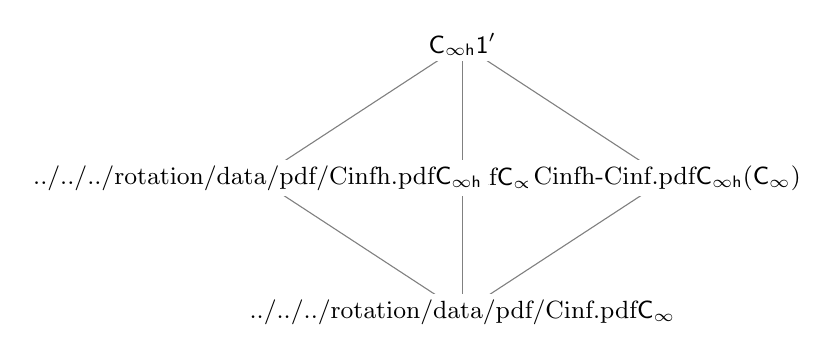
\begin{tikzpicture}[x=1cm, y=1cm, every node/.style={fill=white, font=\small, inner sep=2pt}]
\draw[black!50, line width=0.4pt] (0,0) -- (0,1.7);
\draw[black!50, line width=0.4pt] (0,0) -- (-2.6,1.7);
\draw[black!50, line width=0.4pt] (0,0) -- (2.6,1.7);
\draw[black!50, line width=0.4pt] (0,1.7) -- (0,3.4);
\draw[black!50, line width=0.4pt] (-2.6,1.7) -- (0,3.4);
\draw[black!50, line width=0.4pt] (2.6,1.7) -- (0,3.4);
\node at (0,0) {\href{../../../rotation/data/pdf/Cinf.pdf}{\textcolor{black}{$\grp{C_{\infty}}$}}};
\node at (0,1.7) {\href{Cinf-1p.pdf}{\textcolor{black}{$\grp{C_{\infty}1'}$}}};
\node at (-2.6,1.7) {\href{../../../rotation/data/pdf/Cinfh.pdf}{\textcolor{black}{$\grp{C_{\infty h}}$}}};
\node at (2.6,1.7) {\href{Cinfh-Cinf.pdf}{\textcolor{black}{$\grp{C_{\infty h}}(\grp{C_{\infty}})$}}};
\node at (0,3.4) {\textcolor{black}{$\grp{C_{\infty h}1'}$}};
\end{tikzpicture}\end{center}
The table lists the closed subgroups other than $\grp{C_{\infty h}1'}$ up to conjugacy in $\grp{C_{\infty h}1'}$, one in each row: the continuous subgroups, then those over the members of each family. \label{n:index.family.N}A row with $N$ in its symbol stands for every $N$ of its range, and its entries are functions of $N$. \label{n:head.subgroup}\label{n:head.magnetic.type}\label{n:head.order}\label{n:head.conjugates}\label{n:head.normal}A row gives the representative of a class of subgroups (subgrp), its magnetic type (type), its order, the number of subgroups in the class (conjugates) and whether the representative is normal. \label{n:head.normalizer}\label{n:head.centralizer}It also gives its normalizer and its centralizer in $\grp{C_{\infty h}1'}$. The record holds the members with $N \le 12$ (\texttt{subgroup\symbol{95}classes}), and the section Closed subgroups of the document of \href{../../../rotation/data/pdf/Cinfh.pdf}{$\grp{C_{\infty h}}$} gives other names of some members with $N = 1$.
{\small\begin{longtable}{@{}llrrlll@{}}\toprule
subgrp & type & order & conjugates & normal & normalizer & centralizer\\\midrule\endhead
\bottomrule\endfoot\endlastfoot
\href{../../../rotation/data/pdf/Cinf.pdf}{$\grp{C_{\infty}}$} & I & $\infty$ & 1 & yes & \href{Cinfh-1p.pdf}{$\grp{C_{\infty h}1'}$} & \href{Cinfh-1p.pdf}{$\grp{C_{\infty h}1'}$}\\*
\href{Cinf-1p.pdf}{$\grp{C_{\infty}1'}$} & II & $\infty$ & 1 & yes & \href{Cinfh-1p.pdf}{$\grp{C_{\infty h}1'}$} & \href{Cinfh-1p.pdf}{$\grp{C_{\infty h}1'}$}\\
\href{../../../rotation/data/pdf/Cinfh.pdf}{$\grp{C_{\infty h}}$} & I & $\infty$ & 1 & yes & \href{Cinfh-1p.pdf}{$\grp{C_{\infty h}1'}$} & \href{Cinfh-1p.pdf}{$\grp{C_{\infty h}1'}$}\\
\href{Cinfh-Cinf.pdf}{$\grp{C_{\infty h}}(\grp{C_{\infty}})$} & III & $\infty$ & 1 & yes & \href{Cinfh-1p.pdf}{$\grp{C_{\infty h}1'}$} & \href{Cinfh-1p.pdf}{$\grp{C_{\infty h}1'}$}\\
\grouprule{0pt}{\lightrulewidth}
$\grp{C_{\mathnormal{N}}}$, $N \ge 1$ & I & $N$ & 1 & yes & \href{Cinfh-1p.pdf}{$\grp{C_{\infty h}1'}$} & \href{Cinfh-1p.pdf}{$\grp{C_{\infty h}1'}$}\\
$\grp{C_{\mathnormal{N}}1'}$, $N \ge 1$ & II & $2N$ & 1 & yes & \href{Cinfh-1p.pdf}{$\grp{C_{\infty h}1'}$} & \href{Cinfh-1p.pdf}{$\grp{C_{\infty h}1'}$}\\
$\grp{C_{2\mathnormal{N}}}(\grp{C_{\mathnormal{N}}})$, $N \ge 1$ & III & $2N$ & 1 & yes & \href{Cinfh-1p.pdf}{$\grp{C_{\infty h}1'}$} & \href{Cinfh-1p.pdf}{$\grp{C_{\infty h}1'}$}\\
\grouprule{0pt}{\lightrulewidth}
$\grp{S_{2\mathnormal{N}}}$, $N \ge 1$ & I & $2N$ & 1 & yes & \href{Cinfh-1p.pdf}{$\grp{C_{\infty h}1'}$} & \href{Cinfh-1p.pdf}{$\grp{C_{\infty h}1'}$}\\
$\grp{S_{2\mathnormal{N}}1'}$, $N \ge 1$ & II & $4N$ & 1 & yes & \href{Cinfh-1p.pdf}{$\grp{C_{\infty h}1'}$} & \href{Cinfh-1p.pdf}{$\grp{C_{\infty h}1'}$}\\
$\grp{S_{2\mathnormal{N}}}(\grp{C_{\mathnormal{N}}})$, $N \ge 1$ & III & $2N$ & 1 & yes & \href{Cinfh-1p.pdf}{$\grp{C_{\infty h}1'}$} & \href{Cinfh-1p.pdf}{$\grp{C_{\infty h}1'}$}\\
\grouprule{0pt}{\lightrulewidth}
$\grp{C_{\mathnormal{N}h}}$, $N \ge 1$ & I & $2N$ & 1 & yes & \href{Cinfh-1p.pdf}{$\grp{C_{\infty h}1'}$} & \href{Cinfh-1p.pdf}{$\grp{C_{\infty h}1'}$}\\
$\grp{C_{\mathnormal{N}h}1'}$, $N \ge 1$ & II & $4N$ & 1 & yes & \href{Cinfh-1p.pdf}{$\grp{C_{\infty h}1'}$} & \href{Cinfh-1p.pdf}{$\grp{C_{\infty h}1'}$}\\
$\grp{C_{\mathnormal{N}h}}(\grp{C_{\mathnormal{N}}})$, $N \ge 1$ & III & $2N$ & 1 & yes & \href{Cinfh-1p.pdf}{$\grp{C_{\infty h}1'}$} & \href{Cinfh-1p.pdf}{$\grp{C_{\infty h}1'}$}\\
$\grp{C_{2\mathnormal{N}h}}(\grp{C_{\mathnormal{N}h}})$, $N \ge 1$ & III & $4N$ & 1 & yes & \href{Cinfh-1p.pdf}{$\grp{C_{\infty h}1'}$} & \href{Cinfh-1p.pdf}{$\grp{C_{\infty h}1'}$}\\*
$\grp{C_{2\mathnormal{N}h}}(\grp{S_{2\mathnormal{N}}})$, $N \ge 1$ & III & $4N$ & 1 & yes & \href{Cinfh-1p.pdf}{$\grp{C_{\infty h}1'}$} & \href{Cinfh-1p.pdf}{$\grp{C_{\infty h}1'}$}\\
\bottomrule\end{longtable}}
\needspace{208pt}
\partbox{Angular momentum}
\section{Subduction from \texorpdfstring{$\grp{O(3)1'}$}{O(3)1\unichar{8242}}}\label{s:subduction_o3}
Conventions: \href{../../CONVENTIONS.pdf}{CONVENTIONS.pdf}, sections \href{../../../rotation/CONVENTIONS.pdf\#conv.11}{11}, \href{../../../rotation/CONVENTIONS.pdf\#conv.12}{12}, \href{../../CONVENTIONS.pdf\#conv.33.1}{33.1} and \href{../../CONVENTIONS.pdf\#conv.37.4}{37.4}.
\leavevmode\label{n:index.J}\label{n:index.parity}The irrep $\irrJp{J}{p}$ of $\grp{O(3)1'}$ has angular momentum $J$ and parity $p$ ($\ptag{g}$ for $p = +1$, $\ptag{u}$ for $p = -1$), and time reversal acts on it as on its kets (\href{../../CONVENTIONS.pdf}{CONVENTIONS.pdf}, section \href{../../CONVENTIONS.pdf\#conv.31.1}{31.1}). A corepresentation occurs in its restriction to $\grp{C_{\infty h}1'}$ as often as its first irrep occurs in the restriction to $\grp{C_{\infty h}}$ (the section Subduction from $\grp{O(3)}$ of the document of \href{../../../rotation/data/pdf/Cinfh.pdf}{$\grp{C_{\infty h}}$}). For every $J$,
\begin{equation}\label{e:o3rule}\begin{aligned}\restr{\irrJp{J}{+}}{\grp{C_{\infty h}1'}} &= \irr{a}_{\ptag{g}}\oplus\bigoplus_{n=1}^{J}\conjpair{1}\irr{e}_{n,\ptag{g}}\,\conjpair{2}\irr{e}_{n,\ptag{g}},\\\restr{\irrJp{J}{-}}{\grp{C_{\infty h}1'}} &= \irr{a}_{\ptag{u}}\oplus\bigoplus_{n=1}^{J}\conjpair{1}\irr{e}_{n,\ptag{u}}\,\conjpair{2}\irr{e}_{n,\ptag{u}}.\end{aligned}\end{equation}
A row is an angular momentum $J \le 6$. A row gives the restriction of $\irrJp{J}{p}$ to $\grp{C_{\infty h}1'}$.
\needspace{149pt}
\paragraph{Parity $\ptag{g}$ ($p = +1$).}
{\small\begin{longtable}{@{}rl@{}}\toprule
$J$ & $\restr{\irrJp{J}{+}}{\grp{C_{\infty h}1'}}$\\\midrule\endhead
\bottomrule\endfoot\endlastfoot
0 & $\irr{a}_{\ptag{g}}$\\*
1 & $\irr{a}_{\ptag{g}} \oplus \conjpair{1}\irr{e}_{1\ptag{g}}\,\conjpair{2}\irr{e}_{1\ptag{g}}$\\*
2 & $\irr{a}_{\ptag{g}} \oplus \conjpair{1}\irr{e}_{1\ptag{g}}\,\conjpair{2}\irr{e}_{1\ptag{g}} \oplus \conjpair{1}\irr{e}_{2\ptag{g}}\,\conjpair{2}\irr{e}_{2\ptag{g}}$\\*
3 & $\irr{a}_{\ptag{g}} \oplus \conjpair{1}\irr{e}_{1\ptag{g}}\,\conjpair{2}\irr{e}_{1\ptag{g}} \oplus \conjpair{1}\irr{e}_{2\ptag{g}}\,\conjpair{2}\irr{e}_{2\ptag{g}} \oplus \conjpair{1}\irr{e}_{3\ptag{g}}\,\conjpair{2}\irr{e}_{3\ptag{g}}$\\*
4 & $\irr{a}_{\ptag{g}} \oplus \conjpair{1}\irr{e}_{1\ptag{g}}\,\conjpair{2}\irr{e}_{1\ptag{g}} \oplus \conjpair{1}\irr{e}_{2\ptag{g}}\,\conjpair{2}\irr{e}_{2\ptag{g}} \oplus \conjpair{1}\irr{e}_{3\ptag{g}}\,\conjpair{2}\irr{e}_{3\ptag{g}} \oplus \conjpair{1}\irr{e}_{4\ptag{g}}\,\conjpair{2}\irr{e}_{4\ptag{g}}$\\*
5 & $\irr{a}_{\ptag{g}} \oplus \conjpair{1}\irr{e}_{1\ptag{g}}\,\conjpair{2}\irr{e}_{1\ptag{g}} \oplus \conjpair{1}\irr{e}_{2\ptag{g}}\,\conjpair{2}\irr{e}_{2\ptag{g}} \oplus \conjpair{1}\irr{e}_{3\ptag{g}}\,\conjpair{2}\irr{e}_{3\ptag{g}} \oplus \conjpair{1}\irr{e}_{4\ptag{g}}\,\conjpair{2}\irr{e}_{4\ptag{g}} \oplus \conjpair{1}\irr{e}_{5\ptag{g}}\,\conjpair{2}\irr{e}_{5\ptag{g}}$\\*
6 & $\irr{a}_{\ptag{g}} \oplus \conjpair{1}\irr{e}_{1\ptag{g}}\,\conjpair{2}\irr{e}_{1\ptag{g}} \oplus \conjpair{1}\irr{e}_{2\ptag{g}}\,\conjpair{2}\irr{e}_{2\ptag{g}} \oplus \conjpair{1}\irr{e}_{3\ptag{g}}\,\conjpair{2}\irr{e}_{3\ptag{g}} \oplus \conjpair{1}\irr{e}_{4\ptag{g}}\,\conjpair{2}\irr{e}_{4\ptag{g}} \oplus \conjpair{1}\irr{e}_{5\ptag{g}}\,\conjpair{2}\irr{e}_{5\ptag{g}} \oplus \conjpair{1}\irr{e}_{6\ptag{g}}\,\conjpair{2}\irr{e}_{6\ptag{g}}$\\
\bottomrule\end{longtable}}
\needspace{149pt}
\paragraph{Parity $\ptag{u}$ ($p = -1$).}
{\small\begin{longtable}{@{}rl@{}}\toprule
$J$ & $\restr{\irrJp{J}{-}}{\grp{C_{\infty h}1'}}$\\\midrule\endhead
\bottomrule\endfoot\endlastfoot
0 & $\irr{a}_{\ptag{u}}$\\*
1 & $\irr{a}_{\ptag{u}} \oplus \conjpair{1}\irr{e}_{1\ptag{u}}\,\conjpair{2}\irr{e}_{1\ptag{u}}$\\*
2 & $\irr{a}_{\ptag{u}} \oplus \conjpair{1}\irr{e}_{1\ptag{u}}\,\conjpair{2}\irr{e}_{1\ptag{u}} \oplus \conjpair{1}\irr{e}_{2\ptag{u}}\,\conjpair{2}\irr{e}_{2\ptag{u}}$\\*
3 & $\irr{a}_{\ptag{u}} \oplus \conjpair{1}\irr{e}_{1\ptag{u}}\,\conjpair{2}\irr{e}_{1\ptag{u}} \oplus \conjpair{1}\irr{e}_{2\ptag{u}}\,\conjpair{2}\irr{e}_{2\ptag{u}} \oplus \conjpair{1}\irr{e}_{3\ptag{u}}\,\conjpair{2}\irr{e}_{3\ptag{u}}$\\*
4 & $\irr{a}_{\ptag{u}} \oplus \conjpair{1}\irr{e}_{1\ptag{u}}\,\conjpair{2}\irr{e}_{1\ptag{u}} \oplus \conjpair{1}\irr{e}_{2\ptag{u}}\,\conjpair{2}\irr{e}_{2\ptag{u}} \oplus \conjpair{1}\irr{e}_{3\ptag{u}}\,\conjpair{2}\irr{e}_{3\ptag{u}} \oplus \conjpair{1}\irr{e}_{4\ptag{u}}\,\conjpair{2}\irr{e}_{4\ptag{u}}$\\*
5 & $\irr{a}_{\ptag{u}} \oplus \conjpair{1}\irr{e}_{1\ptag{u}}\,\conjpair{2}\irr{e}_{1\ptag{u}} \oplus \conjpair{1}\irr{e}_{2\ptag{u}}\,\conjpair{2}\irr{e}_{2\ptag{u}} \oplus \conjpair{1}\irr{e}_{3\ptag{u}}\,\conjpair{2}\irr{e}_{3\ptag{u}} \oplus \conjpair{1}\irr{e}_{4\ptag{u}}\,\conjpair{2}\irr{e}_{4\ptag{u}} \oplus \conjpair{1}\irr{e}_{5\ptag{u}}\,\conjpair{2}\irr{e}_{5\ptag{u}}$\\*
6 & $\irr{a}_{\ptag{u}} \oplus \conjpair{1}\irr{e}_{1\ptag{u}}\,\conjpair{2}\irr{e}_{1\ptag{u}} \oplus \conjpair{1}\irr{e}_{2\ptag{u}}\,\conjpair{2}\irr{e}_{2\ptag{u}} \oplus \conjpair{1}\irr{e}_{3\ptag{u}}\,\conjpair{2}\irr{e}_{3\ptag{u}} \oplus \conjpair{1}\irr{e}_{4\ptag{u}}\,\conjpair{2}\irr{e}_{4\ptag{u}} \oplus \conjpair{1}\irr{e}_{5\ptag{u}}\,\conjpair{2}\irr{e}_{5\ptag{u}} \oplus \conjpair{1}\irr{e}_{6\ptag{u}}\,\conjpair{2}\irr{e}_{6\ptag{u}}$\\
\bottomrule\end{longtable}}
\needspace{281pt}
\partbox{Tensors}
\section{Multipoles}\label{s:multipoles}
Conventions: \href{../../CONVENTIONS.pdf}{CONVENTIONS.pdf}, sections \href{../../CONVENTIONS.pdf\#conv.35.1}{35.1} and \href{../../CONVENTIONS.pdf\#conv.37.6}{37.6}.
A row is a rank $J$, and the last row gives every rank (\texttt{every\symbol{95}rank}). \label{n:head.multipole.electric}\label{n:head.multipole.electric.toroidal}A row gives the number of independent multipoles of each kind that $\grp{C_{\infty h}1'}$ allows. It is the multiplicity in $\irrJp{J}{p}$ of the trivial irrep of $\grp{C_{\infty h}}$ (the section Subduction from $\grp{O(3)}$ of the document of \href{../../../rotation/data/pdf/Cinfh.pdf}{$\grp{C_{\infty h}}$}).
{\small\begin{longtable}{@{}rrr@{}}\toprule
$J$ & electric & electric toroidal\\\midrule\endhead
\bottomrule\endfoot\endlastfoot
0 & 1 & 0\\*
1 & 0 & 1\\*
2 & 1 & 0\\*
3 & 0 & 1\\*
4 & 1 & 0\\*
\grouprule{0pt}{\lightrulewidth} every & 1 for $J$ even & 1 for $J$ odd\\
\bottomrule\end{longtable}}
The electric entries at even $J$ count the operators on a spin that $\grp{C_{\infty h}1'}$ allows (\href{../../CONVENTIONS.pdf}{CONVENTIONS.pdf}, section \href{../../CONVENTIONS.pdf\#conv.35.1}{35.1}).
\needspace{103pt}
\section{Invariants}\label{s:invariants}
Conventions: \href{../../CONVENTIONS.pdf}{CONVENTIONS.pdf}, sections \href{../../CONVENTIONS.pdf\#conv.31.2}{31.2} and \href{../../CONVENTIONS.pdf\#conv.35.1}{35.1}.
The invariant polynomials of $\grp{C_{\infty h}1'}$ in one vector of a kind are those of its image of that kind (section~\ref{s:identification}), in the section Invariant polynomials of the image's document (\texttt{rings}).
\leavevmode\label{n:index.degree.polar}\label{n:index.degree.axial}A row is a degree $a$ in a polar vector even under time reversal. A row gives the number of linearly independent invariants of degree $a$ in it and $b$ in an axial vector odd under time reversal, for $a + b \le 6$.
{\small\begin{longtable}{@{}rrrrrr@{}}\toprule
$a$ & $b = 1$ & $b = 2$ & $b = 3$ & $b = 4$ & $b = 5$\\\midrule\endhead
\bottomrule\endfoot\endlastfoot
1 & 0 & 0 & 0 & 0 & 0\\*
2 & 0 & 8 & 0 & 14 & \\*
3 & 0 & 0 & 0 &  & \\*
4 & 0 & 14 &  &  & \\*
5 & 0 &  &  &  & \\
\bottomrule\end{longtable}}
\leavevmode\label{n:local.component.polar}\label{n:local.component.axial}The record holds their bases for $a + b \le 4$ (\texttt{polynomials}), in the components $u_{x}$, $u_{y}$, $u_{z}$ of the polar vector and $v_{x}$, $v_{y}$, $v_{z}$ of the axial vector. \label{n:head.polynomial}A row is an invariant of the reduced row echelon basis of its degrees (\href{../../CONVENTIONS.pdf}{CONVENTIONS.pdf}, section \href{../../CONVENTIONS.pdf\#conv.35.1}{35.1}). A row gives its degrees $a$ and $b$ and the invariant (polynomial).
{\small\renewcommand{\arraystretch}{1.2}\begin{longtable}{@{}rrl@{\hspace{18pt}}rrl@{}}\toprule
$a$ & $b$ & polynomial & $a$ & $b$ & polynomial\\\midrule\endhead
\bottomrule\endfoot\endlastfoot
2 & 2 & $u_{x}^{2}v_{x}^{2} + 2u_{x}u_{y}v_{x}v_{y} + u_{y}^{2}v_{y}^{2}$ & 2 & 2 & $u_{x}u_{z}v_{x}v_{z} + u_{y}u_{z}v_{y}v_{z}$\\*
2 & 2 & $u_{x}^{2}v_{x}v_{y} - u_{x}u_{y}v_{x}^{2} + u_{x}u_{y}v_{y}^{2} - u_{y}^{2}v_{x}v_{y}$ & 2 & 2 & $u_{x}u_{z}v_{y}v_{z} - u_{y}u_{z}v_{x}v_{z}$\\*
2 & 2 & $u_{x}^{2}v_{y}^{2} - 2u_{x}u_{y}v_{x}v_{y} + u_{y}^{2}v_{x}^{2}$ & 2 & 2 & $u_{z}^{2}v_{x}^{2} + u_{z}^{2}v_{y}^{2}$\\*
2 & 2 & $u_{x}^{2}v_{z}^{2} + u_{y}^{2}v_{z}^{2}$ & 2 & 2 & $u_{z}^{2}v_{z}^{2}$\\
\bottomrule\end{longtable}}
\end{document}
